\reportsection{Results and Visualizations}
\subsection{Evaluation rules and metric definitions}
All main test results use the same 1,738 rows. Accuracy is the fraction of correctly predicted labels. For class $k$, precision $P_k$, recall $R_k$, and F1 are
\begin{equation}
P_k=\frac{TP_k}{TP_k+FP_k},\qquad
R_k=\frac{TP_k}{TP_k+FN_k},\qquad
F1_k=\frac{2P_kR_k}{P_k+R_k}.
\end{equation}
Undefined ratios are set to zero. Macro F1 averages $F1_k$ equally across the five label classes. Weighted F1 weights each class by its gold support. For target classification, the macro average uses the 87 distinct gold target strings; guesses outside that set remain wrong predictions. Thus target macro F1 and target accuracy answer different aggregation questions.

JSON category accuracy compares normalized category strings. Target accuracy requires an exact string match. Label accuracy scores only the integer label field. Complete-record accuracy requires category, target, and label to be correct for the \emph{same} example:
\begin{equation}
\operatorname{Acc}_{\mathrm{joint}}=\frac{1}{N}\sum_{i=1}^{N}
\mathbf{1}[\hat c_i=c_i\land\hat t_i=t_i\land\hat y_i=y_i].
\end{equation}
Invalid or missing outputs count as errors rather than being removed. The two canonical JSON test completion files contain valid objects and in-range integer labels for all rows. Their semantic errors therefore cannot be explained solely by JSON parsing failures.

The report independently recomputes metrics from saved prediction CSVs and JSON completions and checks them against the saved evaluation files. For tasks B and C, the canonical SFT results come from the standalone full-test evaluations. Earlier training-time test passes of the same adapters differ by one label prediction and remain in the companion TXT reports. They are repeated evaluations of existing models, not additional SFT models. The incomplete 410-row thinking benchmark and smoke tests are excluded from headline results.

\subsection{Qwen3.5-2B: three tasks, six evaluations}
Table~\ref{tab:qwen} is organized by the task contracts in Table~\ref{tab:contracts}. It compares Base and SFT \emph{within each task}. Every number in this table scores the label. In particular, task B's 93.61\% label accuracy is not its all-fields-correct accuracy.

\begin{table}[H]
\centering\small
\caption{Canonical Qwen test label metrics (\%). Base is the published checkpoint without our task adapter; SFT uses a separate adapter for each task.}
\label{tab:qwen}
\begin{tabular}{llrr}
\toprule Task & State & Label accuracy & Label macro F1\\\midrule
\tableinput{generated/qwen_rows.tex}
\bottomrule
\end{tabular}
\end{table}

\textbf{Task A: sentence to label.} The base checkpoint correctly classifies 403 examples, compared with 1,631 for SFT. Accuracy rises from 23.19\% to 93.84\%, an observed gain of 70.66 percentage points. Macro F1 rises from 14.21\% to 93.89\%. The substantial improvement shows the value of task-specific adaptation under the saved prompt and evaluation protocol. The change also spans a BF16 vLLM base runtime and FP32 adapter runtime, so it should not be read as a controlled numerical-engine ablation.

\textbf{Task B: sentence to all three fields.} The base checkpoint obtains 34.46\% label accuracy and 28.08\% macro F1. The SFT adapter obtains 93.61\% and 93.64\%, respectively. This is an observed label-accuracy gain of 59.15 percentage points. Category, target, and joint correctness are reported separately below.

\textbf{Task C: annotation-conditioned label prediction.} Supplying gold category and target annotations yields 33.54\% base accuracy and 95.51\% SFT accuracy, with macro F1 increasing from 27.63\% to 95.55\%. The accuracy gain is 61.97 percentage points. This is the highest Qwen label score in the recorded runs, but the richer input condition prevents attributing the difference from task A solely to model quality.

\begin{figure}[H]
\centering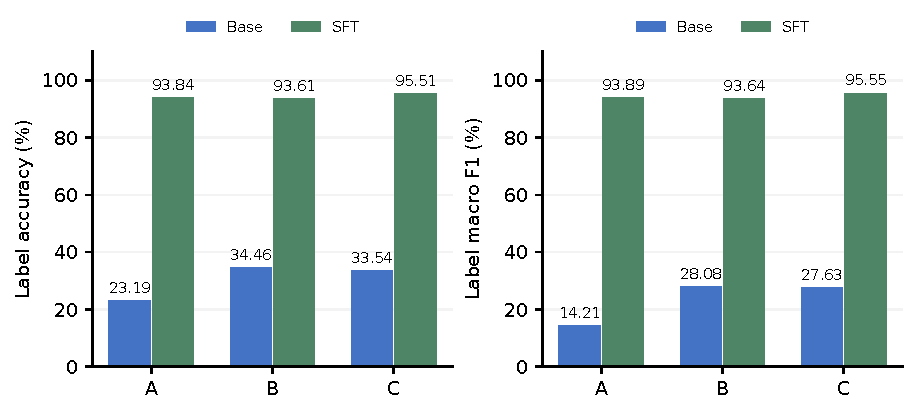
\includegraphics[width=\linewidth]{figures/qwen_task_comparison.pdf}
\caption{Base/SFT comparison for tasks A--C. Both panels score the label; task B's category/target and joint exact-match scores are reported separately.}
\label{fig:qwen}
\end{figure}

\subsection{Structured-output category, target, and joint results}
\begin{table}[H]
\centering\small
\caption{Task B generated-field accuracy and macro F1 (\%). The input is sentence only.}
\label{tab:json}
\begin{tabular}{lrrrr}
\toprule & \multicolumn{2}{c}{Accuracy} & \multicolumn{2}{c}{Macro F1}\\
\cmidrule(lr){2-3}\cmidrule(lr){4-5}
Field & Base & SFT & Base & SFT\\\midrule
\tableinput{generated/json_rows.tex}
\bottomrule
\end{tabular}
\end{table}

The SFT JSON model predicts the category correctly for 1,727 examples and the exact target string for 1,706 examples. It predicts the label correctly for 1,627 examples. Requiring all three fields together leaves 1,614 fully correct examples, or 92.87\%. The corresponding base joint score is 44 correct examples, or 2.53\%. These counts show why a label-only score is insufficient to describe structured-output reliability.

Category macro F1 is 99.48\% after SFT, whereas exact target macro F1 is 97.51\%. The target scores preserve string distinctions such as capitalization and underscores. Base target macro F1 (43.47\%) exceeds its overall target accuracy (21.69\%) because macro F1 weights each target class equally while accuracy weights individual examples. It should not be substituted for exact target accuracy.

\subsection{Encoder results and review-stage reference baselines}
\begin{table}[H]
\centering\small
\caption{Prediction-backed sentence-only encoder test results (\%).}
\label{tab:encoders}
\begin{tabularx}{\linewidth}{Xrr}
\toprule Saved model / run & Accuracy & Macro F1\\\midrule
\tableinput{generated/encoder_rows.tex}
\bottomrule
\end{tabularx}
\end{table}

ModernBERT-base's retuned run improves over its original saved run from 89.36\% to 92.12\% accuracy. The saved ModernBERT-large run reaches 93.33\%, making it the strongest encoder result in this artifact collection. ALBERT obtains 88.09\%. These runs share the sentence-only task, but model size, training duration, schedule, and other hyperparameters vary. The table therefore summarizes observed configurations rather than isolating a single architectural cause.

The review-stage document additionally reports MiniLM accuracy/macro F1 of 77.33\%/74.29\%, Qwen3-Embedding-0.6B of 91.08\%/91.11\%, and an earlier ModernBERT-large review entry of 92.98\%/93.05\%.

\subsection{Confusion matrices and remaining errors}
\begin{figure}[H]
\centering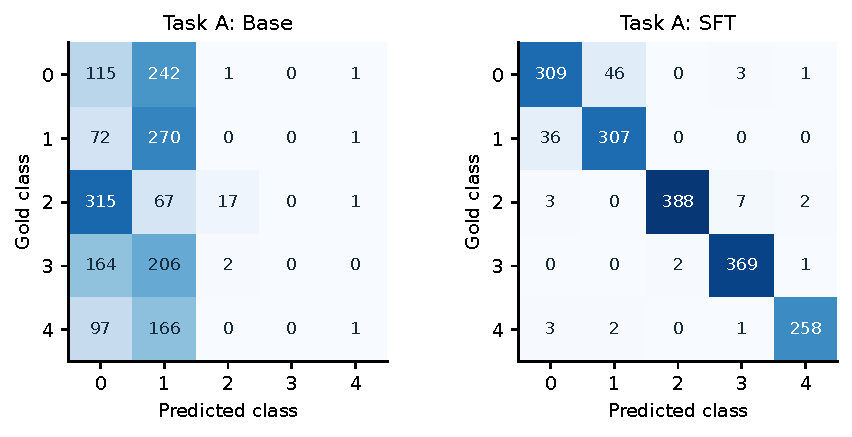
\includegraphics[width=\linewidth]{figures/task_a_confusion.pdf}
\caption{Task-A confusion matrices from the same 1,738 test rows. Rows are gold classes and columns are predicted classes. IDs 0--4 follow Table~\ref{tab:dataset}. Both panels use the same color scale.}
\label{fig:confusion}
\end{figure}

The task-A base checkpoint predicts no class-3 examples correctly and correctly identifies only one bias example. Its predictions concentrate on the stereotype and anti-stereotype classes. This behavior explains why its macro F1 is substantially below its accuracy and demonstrates a mismatch between a general model's prompted decisions and the benchmark label taxonomy.

SFT improves performance across all five classes. The remaining 107 task-A errors include 46 gold anti-stereotypes predicted as stereotypes and 36 gold stereotypes predicted as anti-stereotypes. Together these 82 swaps account for approximately 76.64\% of its mistakes. The two corresponding class F1 scores are 87.04\% and 87.97\%, below the neutral and bias class scores of about 98\%. The explanation examples below examine word-level contributions for individual ModernBERT-large decisions.

\Needspace{.83\textheight}
\subsection{Effect of auxiliary annotations: task A versus task C}
Task A predicts the label from the sentence alone, while task C also receives the gold category and target annotations. Figure~\ref{fig:metadata_confusion} compares these inputs within the Base and SFT states on the same 1,738 test sentences. The SFT panels use the adapter trained for each respective task.

\begin{figure}[H]
\centering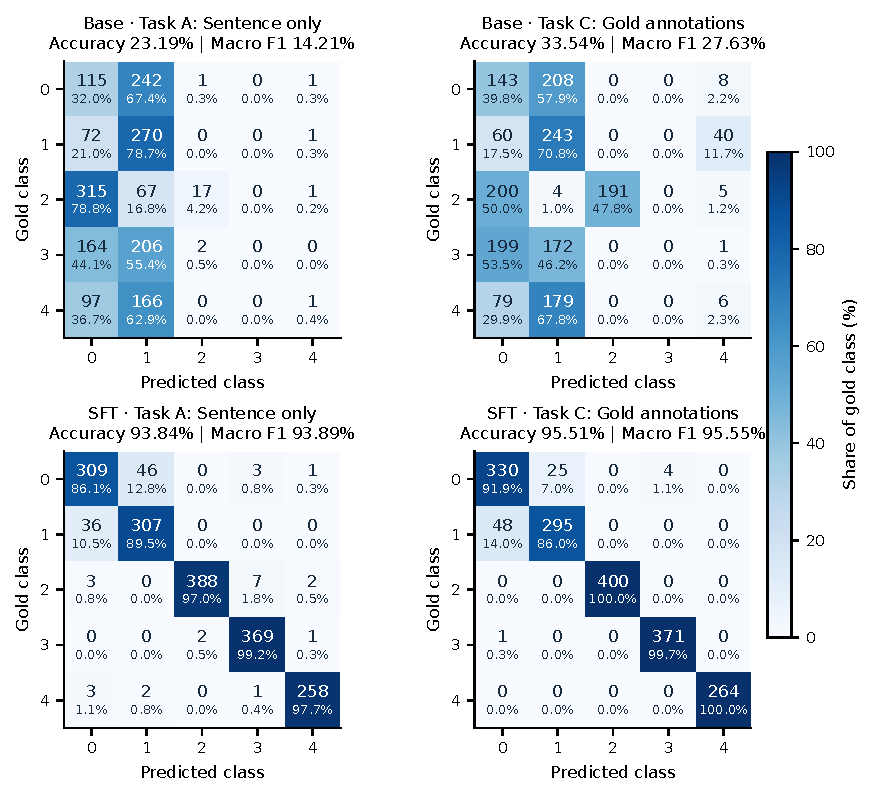
\includegraphics[width=\linewidth]{figures/metadata_confusion_comparison.pdf}
\caption{Task A versus task C: Base models (top) and SFT models (bottom). Each cell shows its count and percentage within the gold-class row. All four panels share the 0--100\% color scale; diagonal percentages are class recall. Class IDs follow Table~\ref{tab:dataset}. Auxiliary annotations are the gold category and target.}
\label{fig:metadata_confusion}
\end{figure}

\begin{table}[H]
\centering\small
\caption{Observed gain from category and target annotations. Accuracy and macro F1 are percentages; gain is in percentage points.}
\label{tab:metadata_gain}
\begin{tabular}{lrrrrr}
\toprule State & A accuracy & C accuracy & Gain (pp) & A macro F1 & C macro F1\\\midrule
\tableinput{generated/metadata_comparison_rows.tex}
\bottomrule
\end{tabular}
\end{table}

For the Base checkpoint, conditioning on category and target annotations increases correct predictions from 403 to 583, raising accuracy from 23.19\% to 33.54\% (+10.36 percentage points). Among the paired predictions, task C corrects 242 task-A errors and changes 62 previously correct answers, giving a net gain of 180. The largest class gain is neutral without target term: its correct count rises from 17 to 191, and recall rises from 4.25\% to 47.75\%.

For SFT, correct predictions increase from 1,631 to 1,660, raising accuracy from 93.84\% to 95.51\% (+1.67 percentage points). Task C corrects 53 task-A errors and changes 24 previously correct answers, giving a net gain of 29. Anti-stereotype recall rises from 86.07\% to 91.92\%; neutral-without-target and bias recall reach 100\%. Stereotype recall changes from 89.50\% to 86.01\%, while its F1 increases from 87.97\% to 88.99\%. The matrices show these class-specific changes alongside the overall gain.

\Needspace{.68\textheight}
\subsection{Explainability example 1: a correct stereotype prediction}
The first saved ModernBERT-large example is test index 1713: \emph{``Producers are businesslike''}. Both the gold label and prediction are class 1 (stereotype). Figure~\ref{fig:explain1} displays the LIME and SHAP values for that predicted class. The word \emph{businesslike} has the largest positive value in both methods: approximately +0.688 for LIME and +0.631 for SHAP. Masking the top-ranked word lowers the predicted class probability by 57.73 percentage points in the saved sensitivity check.

\begin{figure}[H]
\centering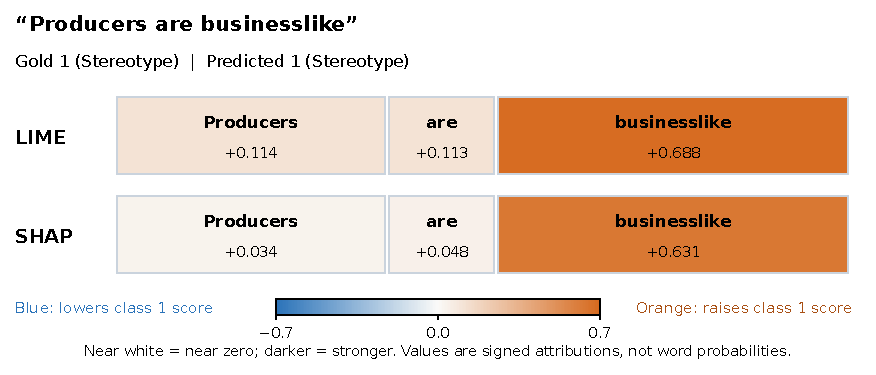
\includegraphics[width=\linewidth]{figures/explanation_1.pdf}
\caption{Correct ModernBERT-large prediction. Orange raises the explained class-1 score, blue lowers it, and near white is close to zero. The shared display range is $[-0.70,+0.70]$.}
\label{fig:explain1}
\end{figure}

This example shows how word-occurrence attributions and masking identify a strong model sensitivity. The displayed contributions are computed for class 1 using this sentence and the configured explanation background.

\Needspace{.68\textheight}
\subsection{Explainability example 2: a misclassified sentence}
The second saved example is test index 1205: \emph{``Gentlemen open the car doors for their date.''} Its gold label is class 4 (bias), while ModernBERT-large predicts class 0 (anti-stereotype). Both rows in Figure~\ref{fig:explain2} therefore explain the \emph{incorrect predicted class 0}, not the gold class. The word \emph{Gentlemen} has the strongest positive support: approximately +0.461 in LIME and +0.370 in SHAP. The strongest negative SHAP contribution is \emph{car}, at approximately $-0.099$.

\begin{figure}[H]
\centering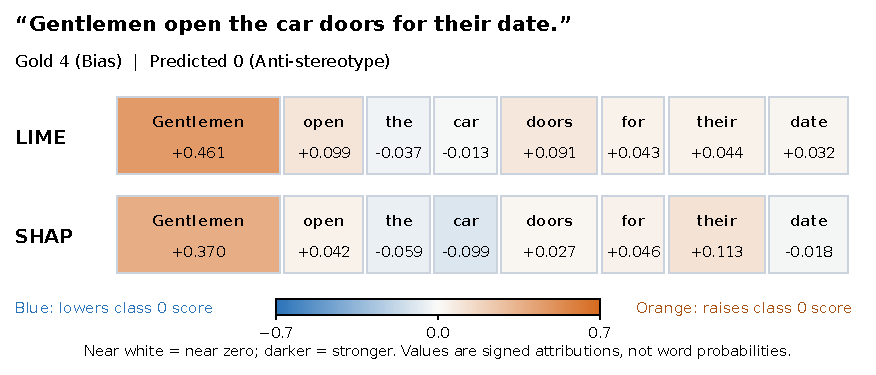
\includegraphics[width=\linewidth]{figures/explanation_2.pdf}
\caption{Misclassified ModernBERT-large example, explaining class 0. The color map and limits are identical to Figure~\ref{fig:explain1}; signs refer to the displayed class, not sentiment or correctness.}
\label{fig:explain2}
\end{figure}

This example illustrates how word attributions can be used to inspect an incorrect decision. Both examples are selected from the saved 100-example diagnostic set.

\subsection{Future Work}
Further experiments can compare training schedules, numerical precision, and batch size across model families. Task-specific comparisons will continue to distinguish sentence-only inputs from annotation-conditioned inputs.

Future work could introduce reinforcement-learning-based fine-tuning with verifiable task rewards to test whether Qwen can better distinguish stereotypes from anti-stereotypes and produce more consistent structured outputs. Rewards could combine label correctness, category and target correctness, and JSON validity; the resulting models should be compared with the current SFT adapters on held-out data.

Additional development can extend structured target prediction and compare exact string matching with semantic matching. The explanation workflow can be expanded with human-reviewed word attributions, perturbation stability studies, and external-domain evaluation.

\subsection{Complete per-class label reports}
The following tables provide precision (P), recall (R), F1, and gold support (N) for the six canonical Qwen evaluations and the four saved encoder runs. P/R/F1 are percentages. Base and SFT belong to their named task contracts; JSON labels come from the generated \code{label} field.

{\small
\begin{longtable}{p{6.8cm}rrrr}
\caption{Full per-class label classification reports.}\label{tab:fullreports}\\
\toprule Class / aggregate & P (\%) & R (\%) & F1 (\%) & N\\\midrule\endfirsthead
\multicolumn{5}{l}{\textit{Table \thetable\ continued}}\\
\toprule Class / aggregate & P (\%) & R (\%) & F1 (\%) & N\\\midrule\endhead
\midrule\multicolumn{5}{r}{\textit{Continued on next page}}\\\endfoot
\bottomrule\endlastfoot
\tableinput{generated/label_reports.tex}
\end{longtable}}

\subsection{Complete category and target reports for task B}
Table~\ref{tab:categoryreport} scores the five normalized categories predicted from sentence-only JSON generation. Table~\ref{tab:targetreport} lists all 87 exact gold target strings. The common support column refers to gold examples. Out-of-set target guesses count as errors and do not create extra classes in the gold-class macro average.

{\scriptsize
\begin{longtable}{lrrrrrrr}
\caption{Task-B category report (\%).}\label{tab:categoryreport}\\
\toprule & \multicolumn{3}{c}{Base} & \multicolumn{3}{c}{SFT} & \\
\cmidrule(lr){2-4}\cmidrule(lr){5-7}
Category & P & R & F1 & P & R & F1 & N\\\midrule\endfirsthead
\toprule Category & Base P & Base R & Base F1 & SFT P & SFT R & SFT F1 & N\\\midrule\endhead
\bottomrule\endlastfoot
\tableinput{generated/category_reports.tex}
\end{longtable}
\begin{longtable}{p{3.5cm}rrrrrrr}
\caption{Task-B target report: all 87 exact target strings (\%).}\label{tab:targetreport}\\
\toprule & \multicolumn{3}{c}{Base} & \multicolumn{3}{c}{SFT} & \\
\cmidrule(lr){2-4}\cmidrule(lr){5-7}
Gold target & P & R & F1 & P & R & F1 & N\\\midrule\endfirsthead
\multicolumn{8}{l}{\textit{Table \thetable\ continued}}\\
\toprule Gold target & Base P & Base R & Base F1 & SFT P & SFT R & SFT F1 & N\\\midrule\endhead
\midrule\multicolumn{8}{r}{\textit{Continued on next page}}\\\endfoot
\bottomrule\endlastfoot
\tableinput{generated/target_reports.tex}
\end{longtable}}
